\section{Auswertung}
\label{sec:Auswertung}
\subsection{Charakteristik des Zählrohrs} % (fold)
\label{sub:charakteristik_aus}

Die Messung wird nach \autoref{sub:charakteristik_durch} durchgeführt. Die Messwerte zu Spannung, Stromstärke und die Zählrate, sowie der Fehler
der Zählrate werden in
\autoref{tab:tab1} aufgetragen.
$N$ ist hierbei schon umgerechnet in Impulse pro Sekunde und der Fehler wird aufgrund der Poissonverteilung nach der Formel
\begin{align*}
  \Delta N &= \sqrt{N} 
\end{align*}
bestimmt.
\begin{table}[H]
  \centering
  \caption{Messwerte zur Bestimmung der Charakteristik des Zählrohrs.}
  \label{tab:tab1}
  \sisetup{table-format=3.2}
  \begin{tabular}{S[table-format=3.0]S[table-format=1.1]S@{${}\pm{}$}S[table-format=2.2]}
  \toprule
   {$U\mathbin{/} \si{\volt}$} &{$ I \mathbin{/} \si{\micro\ampere}$} & \multicolumn{2}{c}{$N \mathbin{/} \frac{Impulse}{\si{\second}}$} \\
  \midrule 
   320 & 0.2 &  106.08 & 10.30 \\
   330 & 0.2 &  109.25 & 10.45 \\
   340 & 0.2 &  109.52 & 10.47 \\
   350 & 0.2 &  110.15 & 10.50 \\
   360 & 0.2 &  111.33 & 10.55 \\ 
   370 & 0.2 &  113.85 & 10.67 \\
   380 & 0.2 &  111.55 & 10.56 \\ 
   390 & 0.2 &  112.40 & 10.60 \\
   400 & 0.2 &  114.37 & 10.69 \\ 
   410 & 0.2 &  111.65 & 10.57 \\
   420 & 0.2 &  113.35 & 10.65 \\ 
   430 & 0.3 &  112.92 & 10.63 \\
   440 & 0.3 &  113.75 & 10.67 \\ 
   450 & 0.3 &  111.25 & 10.55 \\
   460 & 0.4 &  113.18 & 10.64 \\
   470 & 0.4 &  110.13 & 10.49 \\
   480 & 0.4 &  115.18 & 10.73 \\ 
   490 & 0.4 &  114.25 & 10.69 \\
   500 & 0.4 &  115.50 & 10.75 \\ 
   510 & 0.4 &  113.17 & 10.64 \\
   520 & 0.4 &  112.77 & 10.62 \\
   530 & 0.5 &  114.62 & 10.71 \\
   540 & 0.5 &  113.18 & 10.64 \\ 
   550 & 0.5 &  114.90 & 10.72 \\
   560 & 0.5 &  114.75 & 10.71 \\ 
   570 & 0.6 &  115.30 & 10.74 \\
   580 & 0.6 &  115.40 & 10.74 \\ 
   590 & 0.6 &  112.48 & 10.61 \\
   600 & 0.6 &  117.58 & 10.84 \\ 
   610 & 0.6 &  116.65 & 10.80 \\
   620 & 0.7 &  116.95 & 10.81 \\
   630 & 0.7 &  118.35 & 10.88 \\
   640 & 0.7 &  116.77 & 10.81 \\
   650 & 0.7 &  116.97 & 10.81 \\
   660 & 0.6 &  116.48 & 10.79 \\
   670 & 0.7 &  115.98 & 10.77 \\ 
   680 & 0.7 &  117.95 & 10.86 \\
   690 & 0.8 &  119.42 & 10.93 \\
   700 & 0.8 &  120.02 & 10.96 \\
  \bottomrule
  \end{tabular}
\end{table}

Aus den Messwerten wird die Zählrohrcharakteristik graphisch in \autoref{fig:plot1} dargestellt, also die Zählrate N gegenüber der Spannung aufgetragen.
Um den Plateauanstieg zu bestimmen wird zudem mithilfe der Pythonmodule Matplotlib\cite{matplotlib}, Scipy\cite{scipy}, Uncertainties\cite{uncertainties}
und Numpy\cite{numpy} eine Ausgleichsgerade nach $N= aU+b$ bestimmt.
\begin{figure}[H]
  \centering
  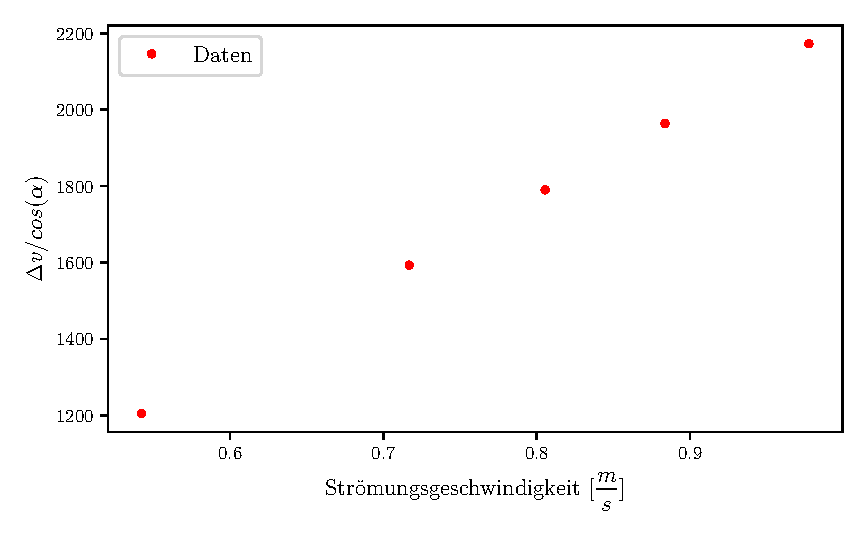
\includegraphics{build/plot1.pdf}
  \caption {Graphische Darstellung der Zählrohrcharakteristik mit Messwerten aus \autoref{tab:tab1}.}
  \label{fig:plot1}
\end{figure}

Die Parameter der linearen Regression betragen
\begin{align*}
  a &= (0.0225 \pm 0.0022)\si{\per\volt}\\
  b &= (102.60 \pm 1.13)\si{\per\second}
\end{align*}

Die Plateaulänge liegt bei $380\si{\volt}$ und 
der relative Plateauanstieg wird zu
\begin{align*}
    a_\text{rel} &= \left( \frac{N(U=\SI{700}{\volt})}{N(U=\SI{320}{\volt})} - 1 \right) \cdot \frac{\SI{100}{\volt}}{(700-320)\:\si{\volt}} \cdot 100 \\
             &= (3.46 \pm 3.97)\si{\percent\per100\volt}
\end{align*}
bestimmt.

\subsection{Totzeit des Zählrohrs}
\label{sub:totzeit_aus}

Wie in \autoref{sub:totzeit_durch} beschrieben, wird die Totzeit des Zählrohrs auf zwei verschiedene Arten bestimmt.
\begin{figure}[H]
  \centering
  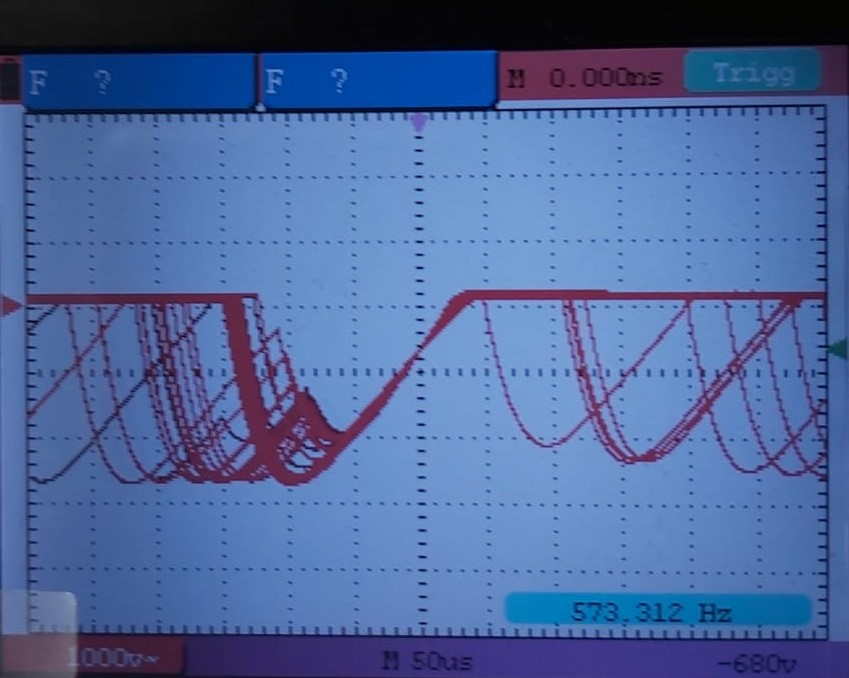
\includegraphics[width=0.7\textwidth]{Abbildungen/Oszilloskop.jpeg}
  \caption {Bildschirmfotos des Oszilloskops zur Abschätzung der Totzeit.}
  \label{fig:Totzeit}
\end{figure}

Aus \autoref{fig:Totzeit} wird die Totzeit
\begin{align*}
  T&= 125 \si{\micro\second}
\end{align*}
abgelesen.

Die Messwerte der Zwei-Quellen-Methode betragen bei einer Messdauer von $t=120\si{\second}$
\begin{align*}
  N_1 &= 87579/120 \si{\per\second}\\
  N_2 &= 126615/120 \si{\per\second}\\
  N_{12} &= 199854/120 \si{\per\second}
\end{align*}

Die Totzeit wird mithilfe von
\begin{align*}
  T&= \frac{N_1+N_2-N_{12}}{2\cdot N_1 \cdot N_2} \label{eqn:totzeit}
\end{align*}
zu 
\begin{align*}
  T_2 &= (78 \pm 36)\si{\micro\second}
\end{align*}
bestimmt.

\subsection{Freigesetzte Ladungen}
\label{sub:ladungen_aus}

Aus den Messwerten kann zusätzlich mithilfe von
\begin{align*}
  Z &= \frac{I}{N*e}
\end{align*}
die Zahl der freigesetzten Ladungen pro detektiertem Teilchen bestimmt werden.
$Z$ ist dabei als Anzahl der Vielfachen der Elementarladung $e= 1,602\cdot 10^{-19}\si{\coulomb}$ angegeben.


Die berechneten Werte sind in \autoref{tab:tab2} eingetragen.

\begin{table}[H]
  \centering
  \caption{Messwerte des Zählrohrs und berechnete Ladung pro einfallendes Teilchen.}
  \label{tab:tab2}
  \sisetup{table-format=3.2}
  \begin{tabular}{S[table-format=3.0]S[table-format=1.1]S@{${}\pm{}$}S[table-format=2.2] S[table-format=1.2]@{${}\pm{}$}S[table-format=1.2]}
  \toprule
   {$U\mathbin{/} \si{\volt}$} &{$ I \mathbin{/} \si{\micro\ampere}$} & \multicolumn{2}{c}{$N \mathbin{/} \frac{Impulse}{\si{\second}}$} &\multicolumn{2}{c}{$Z \mathbin{/} 10^{10} $}\\
  \midrule 
   320 & 0.2 &  106.08 & 10.30 & 1.18 & 0.11 \\
   330 & 0.2 &  109.25 & 10.45 & 1.14 & 0.11 \\
   340 & 0.2 &  109.52 & 10.47 & 1.14 & 0.11 \\
   350 & 0.2 &  110.15 & 10.50 & 1.13 & 0.11 \\
   360 & 0.2 &  111.33 & 10.55 & 1.12 & 0.11 \\ 
   370 & 0.2 &  113.85 & 10.67 & 1.10 & 0.10 \\
   380 & 0.2 &  111.55 & 10.56 & 1.12 & 0.11 \\ 
   390 & 0.2 &  112.40 & 10.60 & 1.11 & 0.10 \\
   400 & 0.2 &  114.37 & 10.69 & 1.09 & 0.10 \\ 
   410 & 0.2 &  111.65 & 10.57 & 1.12 & 0.11 \\
   420 & 0.2 &  113.35 & 10.65 & 1.10 & 0.10 \\ 
   430 & 0.3 &  112.92 & 10.63 & 1.66 & 0.16 \\
   440 & 0.3 &  113.75 & 10.67 & 1.65 & 0.15 \\ 
   450 & 0.3 &  111.25 & 10.55 & 1.68 & 0.16 \\
   460 & 0.4 &  113.18 & 10.64 & 2.21 & 0.21 \\
   470 & 0.4 &  110.13 & 10.49 & 2.27 & 0.22 \\
   480 & 0.4 &  115.18 & 10.73 & 2.17 & 0.20 \\ 
   490 & 0.4 &  114.25 & 10.69 & 2.19 & 0.20 \\
   500 & 0.4 &  115.50 & 10.75 & 2.16 & 0.20 \\ 
   510 & 0.4 &  113.17 & 10.64 & 2.21 & 0.21 \\
   520 & 0.4 &  112.77 & 10.62 & 2.21 & 0.21 \\
   530 & 0.5 &  114.62 & 10.71 & 2.72 & 0.25 \\
   540 & 0.5 &  113.18 & 10.64 & 2.76 & 0.26 \\ 
   550 & 0.5 &  114.90 & 10.72 & 2.72 & 0.25 \\
   560 & 0.5 &  114.75 & 10.71 & 2.72 & 0.25 \\ 
   570 & 0.6 &  115.30 & 10.74 & 3.25 & 0.30 \\
   580 & 0.6 &  115.40 & 10.74 & 3.25 & 0.30 \\ 
   590 & 0.6 &  112.48 & 10.61 & 3.33 & 0.31 \\
   600 & 0.6 &  117.58 & 10.84 & 3.19 & 0.30 \\ 
   610 & 0.6 &  116.65 & 10.80 & 3.21 & 0.30 \\
   620 & 0.7 &  116.95 & 10.81 & 3.74 & 0.35 \\
   630 & 0.7 &  118.35 & 10.88 & 3.69 & 0.34 \\
   640 & 0.7 &  116.77 & 10.81 & 3.74 & 0.35 \\
   650 & 0.7 &  116.97 & 10.81 & 3.74 & 0.35 \\
   660 & 0.6 &  116.48 & 10.79 & 3.22 & 0.30 \\
   670 & 0.7 &  115.98 & 10.77 & 3.77 & 0.35 \\ 
   680 & 0.7 &  117.95 & 10.86 & 3.70 & 0.34 \\
   690 & 0.8 &  119.42 & 10.93 & 4.18 & 0.38 \\
   700 & 0.8 &  120.02 & 10.96 & 4.16 & 0.38 \\
  \bottomrule
  \end{tabular}
\end{table}

In \autoref{fig:plot2} wird $Z$ gegenüber der anliegenden Spannung aufgetragen.
\begin{figure}[H]
  \centering
  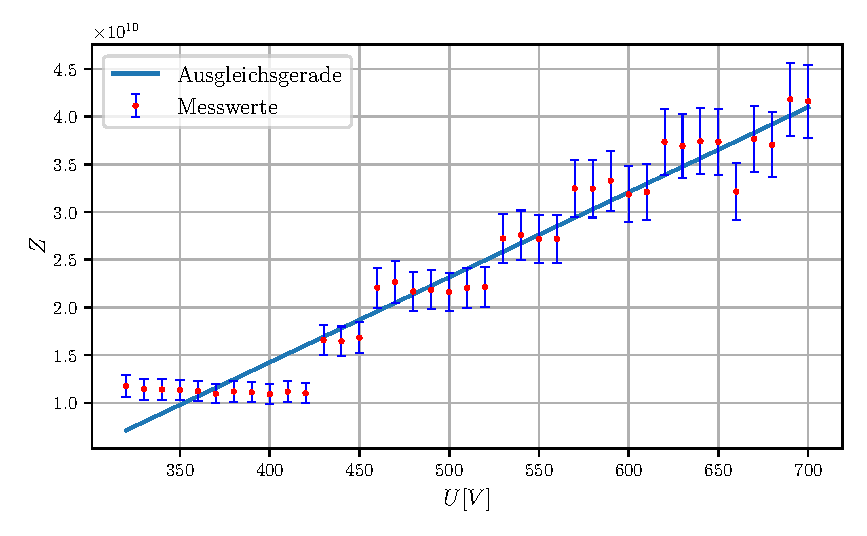
\includegraphics{build/plot2.pdf}
  \caption {Freigesetzte Ladungen pro Teilchen gegenüber der anliegenden Spannung.}
  \label{fig:plot2}
\end{figure}


